\chapter{Основная часть}
\label{cha:design}

\section{Формализованная постановка задачи}
Для выполнения работы необходимо формализовать задачу анализа активности пользователей САПР. Поставленная задача представлена в нотации IDEF0 на рисунке \ref{idef0}. На вход программе подаются информация о выполненных командах и пользовательские параметры: минимальный уровень поддержки, минимальный и максимальный разрывы между командами. Используя методы поиска последовательных шаблонов система определяет часто встречающиеся последовательности команд.

\begin{figure}[h!]
	\centering
	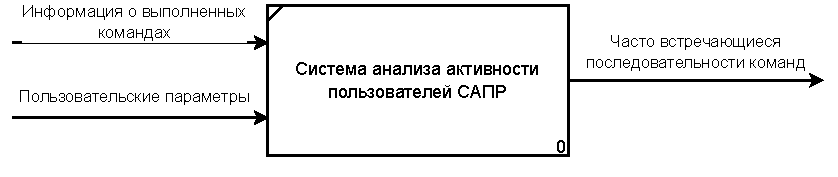
\includegraphics[width=1.0\textwidth]{inc/img/IDEF0.drawio.pdf}
	\caption{IDEF0-диаграмма нулевого уровня}
	\label{idef0}
\end{figure}

\section{Входные и выходные данные}
Данная программа разрабатывается для анализа логов САПР NanoCAD, которые имеют следующий вид: каждая строчка, содержащая действие, начинается с даты и времени выполнения. Начало каждой команды обозначается ее названием, заключенной в символы '<' и '>'. Завершение команды обозначается аналогично, но перед названием команды добавляется символ '/'.

Также поддерживается считывание обезличенных логов, которые не содержат информации о параметрах команд, включая время выполнения. В таком случае время выполнения для каждой команды в сессии будет выставлено автоматически, начиная с 0, увеличивая это значения на 1 для каждой следующей команды.

Кроме этого на вход программе подаются минимальный уровень поддержки, а также минимальный и максимальный разрывы между командами.

На выходе программа выдает часто встречающиеся последовательности команд, их уровни поддержки и коэффициент зависимости.
Коэффициент зависимости показывает насколько команды в последовательности зависят друг от друга и считается как отношение поддержки последовательности к произведению поддержек всех подпоследовательностей состоящих из 1 команды. Если значение коэффициента <= 1, значит зависимости нету. Если же > 1, то зависимость есть. Чем больше единицы, тем вероятней то, что эти команды использовались вместе.

\section{Реализация}
%Разработать программное обеспечение, реализующее описанный метод
За преобразование логов из текста в таблицу базы данных отвечает класс \textit{LogReader}.
%реализованный по паттерну Singleton.
Он может считать все файлы с расширением *.log в выбранной директории и её поддиректориях, записывая все команды в таблицу logs для выбранной на текущий момент базы данных. Также можно указать, нужно ли учитывать завершение команды как отдельное действие, если она началась и закончилась одновременно.

За взаимодействие с базами данных отвечает класс \textit{DataBase}.
%, также реализованный в соответствии с паттерном Singleton.
Данный класс позволяет создавать базы данных,
%(которые являются файлами с расширением *.sqlite),
переключаться между ними и как записывать в них необходимые данные, так и считывать их.

За реализацию разрабатываемого метода отвечает
%отдельный класс.
класс \textit{Calculator}.
Он хранит входные параметры метода, а также необходимые для работы данные и последний полученный результат.

%Добавить ссылку на приложение, где показаны .h файлы этих классов
 Описание данных классов приведено в приложении А.

%Нужно ли писать про UI? Да
%Основное взаимодействия пользователя с программой производится через главное окно.

%\newpage
Пользовательский интерфейс состоит из 4-ех окон. \textit{MainWindow} -- основное окно в котором можно выбирать и просматривать базу данных, считывать в нее логи из выбранной директории, настраивать режимы считывания, задавать параметры метода, запускать его для текущей базы данных и наблюдать результат. \textit{DataBaseWindow} и \textit{ResWindow} используются для просмотра базы данных и результатов работы программы в отдельных окнах. Последнее окно \textit{CmdListWindow} содержит расширенные настройки, в котором можно указать команды которые будут игнорироваться и которые означают начало новой сессии.

Интерфейс программы см. в приложении Б.

%\chapter{Сравнительный анализ времени выполнения этапов метода}
%\label{cha:research}

\section{Сравнительный анализ времени выполнения этапов метода}

%Характеристики устройства, на котором были проведены эксперименты при помощи разработанного ПО: Windows 10 (64-разрядная), 32 GB ОЗУ, i7-7700K.
Чтобы провести сравнительный анализ времени выполнения этапов метода, замерялось их время выполнения с разными значениями минимальной поддержки
и количеством записей
1000 раз, а затем делилось на количество замеров.
Параметр min\_gap был равен нулю, а max\_gap имел максимально возможное значение
%На рисунках \ref{gen_count_60k}-\ref{gen_count_1k} представлены результаты
На рисунке \ref{gen_count_60k} представлен результат
исследования в виде графиков.

%\newpage
\begin{figure}
	\begin{tikzpicture}
		\begin{axis}[
			xlabel={Значение параметра min\_sup},
			ylabel={Время выполнения, сек.},
			xtick={0.10,0.09,0.08,0.07,0.06,0.05,0.04,0.03,0.02,0.01},
			every x tick label/.append style  =
			{ 
				/pgf/number format/.cd,
				precision = 2, 
				fixed
			},
			x dir=reverse,
			legend pos=north west,
			ymajorgrids=true,
			grid style=dashed,
			width = 400,
			]
			
			\addplot[
			color=green,
			mark=halfcircle,
			line width = 1,
			dashed,
			]
			coordinates {
				(0.1, 0.000373886)(0.09, 0.000386969)(0.08, 0.000392265)(0.07, 0.000473179)(0.06, 0.000564197)(0.05, 0.000684211)(0.04, 0.000867599)(0.03, 0.0013237)(0.02, 0.00413822)(0.01, 0.125315)
			};
			\addlegendentry{Генерация кандидатов}
			
			\addplot[
			color=red,
			mark=triangle,
			line width = 1,
			]
			coordinates {
				(0.1, 0.375998)(0.09, 0.382248)(0.08, 0.382072)(0.07, 0.408854)(0.06, 0.436306)(0.05, 0.472805)(0.04, 0.528943)(0.03, 0.63806)(0.02, 1.02797)(0.01, 4.45521)
			};
			\addlegendentry{Подсчет поддержки}
			
		\end{axis}
	\end{tikzpicture}
	\caption{Зависимость времени выполнения разных этапов метода от минимальной поддержки для 66788 записей}
	\label{gen_count_60k}
\end{figure}

%\newpage
%\section*{Вывод из исследовательского раздела}
%В данном разделе был проведен анализ времени выполнения этапов метода.
В результате анализа, можно сделать вывод, что подсчет поддержки кандидатов занимает большую часть времени, чем их генерация.